\subsection{Prototype model}
Ud fra vores vision om et receptfornyelsesmodul og vores MoSCoW prioriteringer, har vi udviklet nedenstående ER-diagram over vores domæne:\\
\begin{center}
	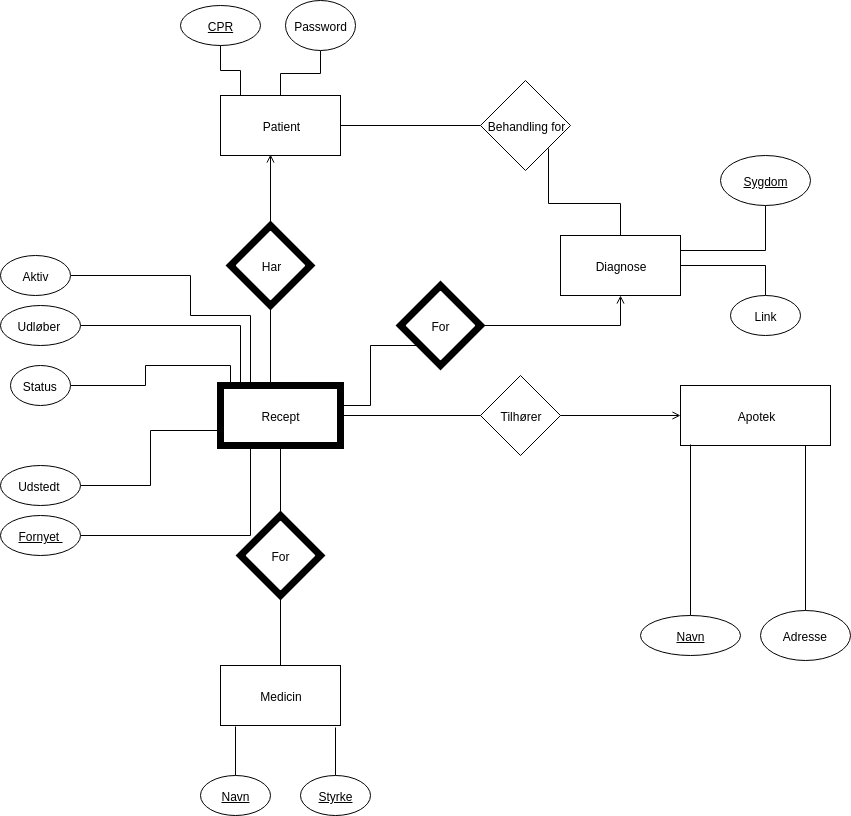
\includegraphics[scale=0.48]{Materials/Prototype/NewERDiagram}
\end{center}
Vores 'recept' entitet kan delvist unikt identificeres ud fra vores andre entiteters nøgler, og er derfor lavet til en weak entity.
Blandt vores ønskede funktioner er historik og medicinkort. For at implementere en historik-funktion, har det været nødvendigt at tilføje en 'Aktiv' attribut til 'recept' entiteten for at skelne mellem tidligere og nuværende recepter. Ved at lave en query på alle recepter, som tilhører et specifikt CPR-nummer, kan vi finde brugerens historik, mens at vi ved at lave en query på et CPR-nummer og angive 'Aktiv' attributten som sand, finder vi de aktive recepter for patienten.\\
Medicinkortet kan ligeledes konstrueres ud fra 'recept' entiteten samt hvilken patient, som ønsker at se sit medicinkort.\\ 
Det har derfor ikke været nødvendigt at lave entiteter til disse features.\\

Vi har herefter omsat vores entiteter til tabeller på samme vis som beskrevet i \textit{'Database Systems. The Complete Book'}\footnote{Prentice Hall, Database Systems. The Complete Book, s. 157-163}. Mange af vores entiteter kan laves direkte til tabeller, som ses nedenfor:
\begin{align*}
	&\textrm{Patient}(\textrm{\underline{CPR}, Password})\\
	&\textrm{Apotek}(\textrm{\underline{Navn}, Addresse})\\
	&\textrm{Medicin}(\textrm{\underline{Navn}, \underline{Styrke}})\\
\end{align*}
Ligeledes kan 'Diagnose' laves direkte. Denne tabel vil komme til at indeholde alle de diagnoser, som kan gives, og er nødvendig, da en patient kan have mere end én diagnose. Et link til patienthåndbogen for hver diagnose gemmes også.
\begin{equation*}
\textrm{Diagnose}(\textrm{\underline{Sygdom}, Link})
\end{equation*}
Vi har herefter vores 'Recept' entitet. Denne er weak og henter nøgler fra de medicin og patient entiteterne. 'Status'-attributten vil blive benyttet i overensstemmelse med vores vision om, at patienten selv skal kunne følge med i receptfornyelsesprocessen. 'Udstedt'-attributten vil blive benyttet af medicinkortet og vil aldrig ændre sig, da den repræsenterer, hvornår patienter første gang blev ordineret med medicinen. 'Udløber'-attributten vil blive benyttet til at sende reminders til patienterne. 'Udløber' og 'Fornyet' attributterne bruges i vores businnes-logic til at afgøre, om en patient kan fornye sin recept, da disse attributter sammen bruges til at bestemme, om der er under x antal dage til, at patientens medicin løber tør. 
\begin{equation*}
	\textrm{Recept}(\textrm{\underline{MedNavn}, \underline{MedStyrke}, \underline{PatCPR}, \underline{sygdom}, \underline{fornyet}, ApoNavn, status, udstedt, udløber, aktiv})
\end{equation*}
Hvis vi skulle lave vores relationer om til tabeller, ville der blive en masse redundancy, da alle på nær en enkelt relation allerede vil være subsets af andre tabeller. Derfor er den eneste relation som bliver lavet om til en tabel 'Behandles for'. Her vil begge nøgler være foreign keys til henholdsvis 'Patient' og 'Diagnose'.
\begin{equation*}
\textrm{BehandlesFor}(\textrm{\underline{PatCPR}, \underline{Sygdom}})
\end{equation*}
Da samtlige danskere har adgang til Min Sundhedsplatform\footnote{Var tilfældet ved projektets begyndelse.} skal der opbevares store mængder af data. Vi mener derfor det er vigtigere at reducere redundancy end at kunne levere hurtige queries. Vi kan undgå redundancy ved at normalisere alle vores tabeller til BCNF. Kigger vi på tabellerne ser vi at de fleste tabeller kun har to attributter. Da enten begge attributter udgør deres key, eller den ene attribut har en functional dependancy over i den anden attribut, har vi at de eneste functional dependancies i disse tabeller er key constraints, og disse er altså trivielt i BCNF.\\
Vi kan identificere en recept unikt gennem 'MedNavn', 'MedStyrke', 'PatCPR', 'Sygdom' og 'Fornyet'. Dette betyder at vi har en functional dependancy:
\begin{equation*}
	\textrm{MedNavn, MedStyrke, PatCPR, Sygdom, Fornyet} \to \textrm{ApoNavn, Status, Udstedt, Udløber, Aktiv}
\end{equation*}
Attributten 'Fornyet', kan give 'Udløber'. Men vi vurderer, at hvis lægen selv indskriver en udløbsdato på recepterne, vil det give lægen mere fleksibilitet i systemet til at tilpasse behandlinger. Dette vil betyde at ovennævnte functional dependancy er den eneste, og da det er en key constraint er 'Recept' i BCNF. 

